\chapter{Implementation of the mem-HNN}

\section{Zielsetzung und Forschungsmethodik}
Upon establishing the precise research methodology, this chapter delves into the practical application of the previously mentioned methods.
First, the analysis phase of the \ac{DSR} process is executed with the goal to establish a model of the research plan 
which the requirements and framework conditions of the \ac{IT}-solution can be derived from. 
Next, the practical implementation is performed during the iterative design phase and uses the method of prototyping.
In the end of the design phase is a functional \ac{IT}-artifact, which fulfills the set requirements.
The evaluation phase in this chapter uses the method of simulation to answer the second part of the research question; to see how efficient 
the \ac{mem-HNN} can utilize the AI-model in terms of throughput and energy usage.

\section{Analysis phase}
\subsection{General conditions}
The first phase of the \ac{DSR}-cycle has the goal of specifying the objective and establishing an according research outline and the requirements of the artifact.
Additionally, the research outline should be visualized as a model of the overall solution concept.\footcite[cf.][278-279]{oesterleKonsortialforschung2010}
The objective of the practical part is already specified in chapter 3.1.
The underlying motivation hereby is to research if the known proof of concepts are feasible on the complete \ac{mem-HNN}
and evaluate if that brings an actual acceleration, which is equivalent to answering the research question of this thesis. 
This is tested by implementing the concept in software that is also part of the ASIC design process.\footnote{cf.\cite{raoUltimateGuideASIC}, p. 1; cf.\cite{ASICDesignFlow}, p. 1}

The implementaton is executed in the programming language Python since it offers a variety of third party libraries that are useful 
for machine learning that are state of the art, like pytorch, scikit learn etc..\footcite[cf.][306-307]{DiscreteContinuousModels}
Furthermore, sciki learn is chosen as machine learning library since it is the one of the industry standards for classical machine learning, has a broad variety of features in terms of \ac{RBM}s
and has a lower learning curve compared with e.g. Tensorflow.\footcite[cf.][5-6]{raschkaMachineLearningPython2020}

It should also be clarified that the hardware, which the analog \ac{mem-HNN}-accelerator consists of, is implemented in software. 
This design decision is made out of time constraints of this thesis and part of the ASIC design process before buildng an actual accelerator. 
Nonetheless, the complete hardware is realizable in software without taking compromisses within their functionality.
The simulation data gathered later on is close to the actual energy efficiency and throughput.QUELLE FEHLT. 

\subsection{Requirements}

In order to set requirements for the IT-artifact the overall solution architecture is of importance. 
Hence, a complete solution is modelled, which surpasses both proof of concepts introduced in 2.4.4.
This solution, visualized in the following figure\ref{Overall architecture}, contains the interaction between the digital computer and the analog mem-HNN Accelerator with five different steps. 
\begin{figure}[H]
    \centering
    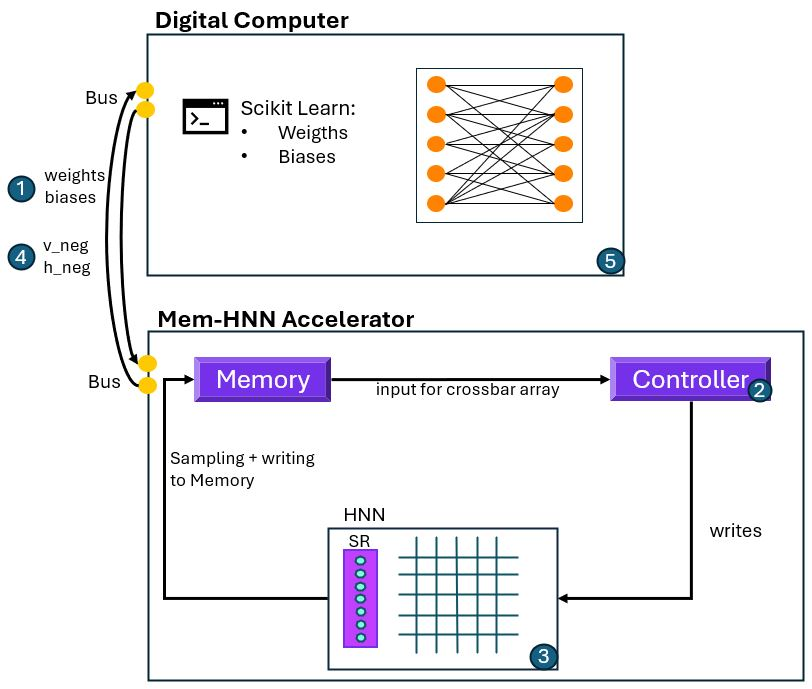
\includegraphics[width=0.80\linewidth]{graphics/Analysemodell.JPG}
    \caption{proposed solution architecture}
    \label{Overall architecture}
\end{figure}
\textbf{1.} contains the initialization of the neural network. 
Hence, the weights and biases are assigned and the structure is build.

\textbf{2.} starts with the transfer of the weigths and biases to the \ac{mem-HNN} accelerator via a bus-system. 
The local memory saves the data and forwards them to the controller. 
The controller is able to programm the memristors in the crossbar array, communicates with the computer and sets a counter and reset for the amount of sampling steps. 

\textbf{3.} is the Hopfield Neural Network (HNN), which contains the memristor crossbar array and the state register (SR).
The state register includes the current neuron configuration.\footcite[cf.][18]{caiHarnessingIntrinsicNoise2019}
For each of the neurons a \ac{TIA} and comparator are required in the hardware.
Furthermore, the state register can lock und unlock specific neurons, so that it is possible to update neurons synchronously.
This enables the possibility of the promissing N/2 update strategy.

\textbf{4.} After iterating over steps two and three multiple times until enough sampling are executed the, all the configurations
of the visible neurons \(v_{neg}\) and the  hidden neurons \(h_{neg}\) are transferred from the controller via the bus-system to
the digital computer. 

\textbf{5.} contains the update of the weights and biases. 
Furthermore, the model can be evaluated in its performance in terms of chosen metrics like prediction accuracy or the negative likelihood etc..
In this case a logistic regression is used for the classification task and the \ac{RBM} is used for the trainng of the neural network. 
After the evaluation the iteration is completed and the new weghts and biases can be transmitted for the following training iteration.

With this underlying model deriving the requirements is the next step in establishing the research outline.
The aim of generating requirements is to generate good quality, not perfect, requirements that offers an acceptable level of risk to start the project.\footcite[cf.][11]{ebertSystematischesRequirementsEngineering2008}
Hence, these requirements need to cover the functions of the \ac{mem-HNN}, which then must be implemented by the respective software components.
Despite this, requirements may evolve over time and occasionally require adjustments when outcomes differ from initial expectations.
As a result, the analysis of the model in conjunction with the reasearch question and under thought of the defined objective, the following requirements for the software emerged:
\textbf{Digital Computer}
\begin{itemize}
    \item Defining a \ac{RBM}
    \item Utilization of any training data
    \item Training a \ac{RBM}
    \item Establishing a pipeline for the classification
    \item Possibility of conventional sampling algorithms: gibbs sampling and metropolis hasting
    \item Setting individual parameters: sampling steps, training iterations 
\end{itemize}
\textbf{Simulated Mem-HNN Accelerator}
\begin{itemize}
    \item Using any \ac{RBM} as input
    \item Correctly using the Hopfield Network update algorithm
    \begin{itemize}
        \item Imitating the hopfield activation function 
        \item Drawing random neurons to update 
        \item Correct injection of the gaussian noise scale
        \item Calculating the weighted sum 
        \item Comparing the weighted sum + bias + noise agaisnt the threshold
        \item Saving the new neuron configuration
    \end{itemize}
    \item Return sampled output of the neuron configurations 
    \item Possibility to use N/2 half updating method instead of asynchronously update of states
    \item Component for measuring the parameters required for evaluation: Speed (throughput) and energy consumption
\end{itemize}
Fruthermore, the python program should be split logically into the different modules and components to enable well structured code. 
With set requirements it is now possible to begin the iterative design and evaluation cycle with focusing on some requirements per iteration.

\section{Design phase}-




-Testen der Aktivierungsfunktion, wenn ich ein Neuron trainiere und dann Mitteln 
- Von vornerein auf Netzwerk Basis arbeiten mit mehren Neuron, jedoch für 1 Neuron testen



Hopfield Netzwerk aktivierungsfunktion der Updating methode

-> Konzeptionell Art des Updates mit keiner Temperatur wie bei MCMC 
Unterschied von MCMC zu Hopfield Netzwerk -> Zufällige Konfiguration und minimale Energie finden. Jedoch hat ein Hopfield
Netzwerk keine Temperatur 

-> Starte zufällige Konfiguration
-> Wähle ein Neuron aus und Berechne Summe und addiere mit Bias, 
-> Update wenn thresshold überschritten 1 und dann auf 0 
-> Speichern der neuen Konfuguration 
-> Starte iteration von gespeicherter Konfiguration 
-> Am Ende habe ich 10000 Vektoren (Die Konfigurationen) -> V1 Neuron wurde so und so oft aktiviert und ich muss average
über das neuron und habe dadurch die Aktivierungswarscheinlichkeit.

-Aktivierungsfunktion einfügen (Binary Step und verfleich zu sigmoid von Abb.4)



\section{Evaluation phase}

Aufbau der Simulator Pipeline
KI-Bibliothek Scikit-Learn
Evaluationsphase

To integrate simulation into the DSR concept ... 
The desired result of the prototyping is completing the \ac{DSR} design phase and with a simulation the result should be verified.
The input is the finished prototype, that mirrors the functionalities of the \ac{ASIC} on a high level.
